\subsection{Linienbreite als Funktion der Ein-/Ausgangsspaltbreite}

Ein entscheidender Faktor bei der Spektroskopie ist die Breite des Eingangs- und Ausgangsspaltes. Diese beeinflusst unteranderem maßgeblich die Breite, 
in der die Linien erscheinen. Deutlich wird dies in Grafik \ref{LinVergleich}. In dieser wurden die auf Eins normierten Linien gleichzeitig dargestellt. 
Man sieht schön, dass bei breiteren Ein- und Ausgangsspalten auch die Linien breiter werden. Dies war auch zu erwarten, da sowohl bei rechteckigem als auch bei 
dem gaußförmigen Intensitätsprofil, die Linienbreite direkt proportional zu den Spaltbreiten ist.
\begin{figure}[h]
    \centering
    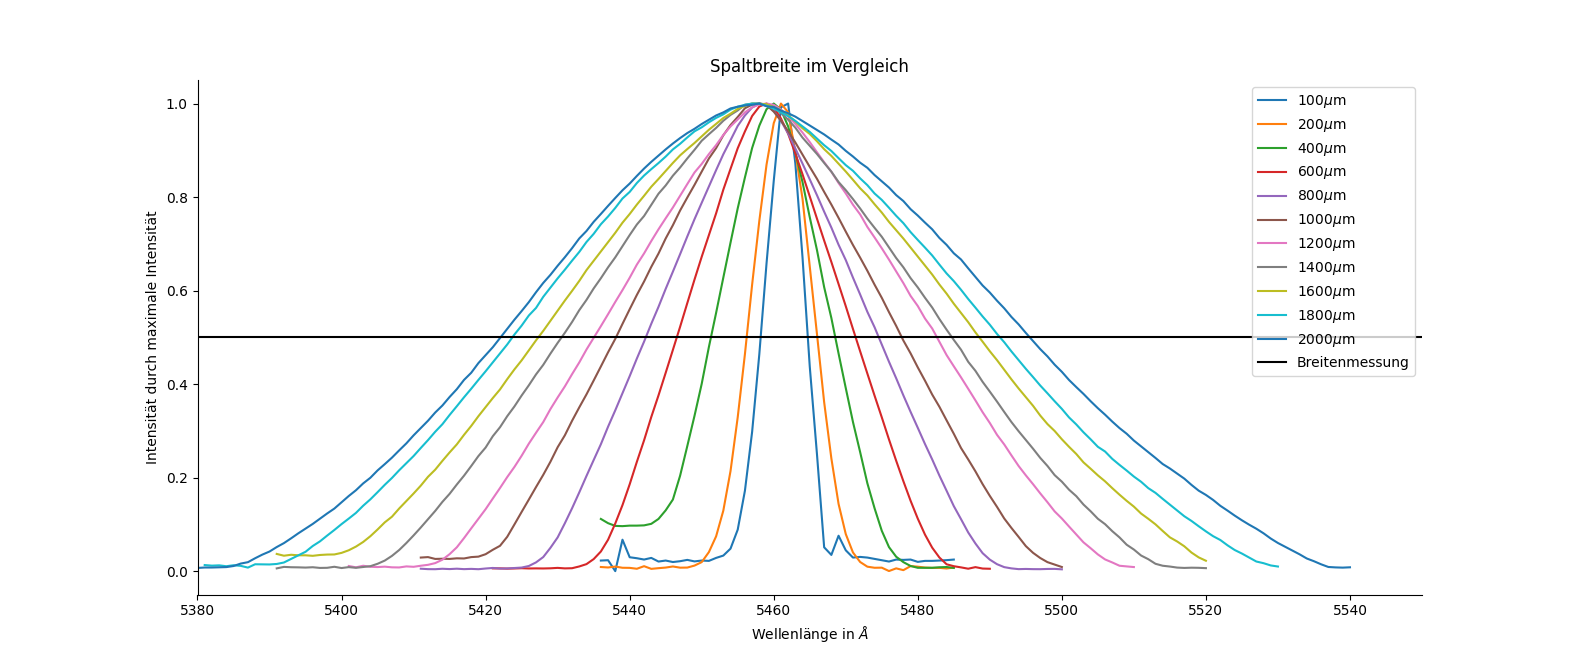
\includegraphics[width = \linewidth]{Bilder/LinienbreiteVergleich.png}
    \caption{Linienbreiten im Vergleich}
    \label{LinVergleich}
\end{figure}
Die schwarze Linie mit dem Namen „Breitenmessung“ dient der Verdeutlichung der Auswertmethodik. Hier wurde grafisch ausgewertet. Um das Problem zu umgehen, 
zu entscheiden, wo genau die Linie bei Null beginnt, nimmt man sie einfach bei halber Intensität die Linienbreite. 
Dies vergrößert jedoch den Fehler, da die Ablesegenauigkeit durch die Auflösung der Grafik begrenzt ist.\\
Beim Auswerten der Grafik ergeben sich folgende Linienbreiten:
\begin{table}[h]
    \centering
    \begin{tabular}[h]{c|c|c|c}
        Spaltbreite in $\mu$m & Linienbreite $\Delta \lambda $ in \r{A} & Fehler $s_{\Delta \lambda }$ in \r{a}& Reale Linienbreite in \r{A}\\
        \hline
        100 & 6.5573 & 0.8 & 5.6477\\
        200 & 9.8360 & 0.8 & 7.2345\\
        400 & 18.0327 & 0.8 & 12.1468\\
        600 & 25.4098 & 0.8 & 15.6837\\
        800 & 31.9672 & 0.8 & 17.6454\\
        1000 & 40.9836 & 0.8 & 23.8628\\
        1200 & 48.3606 & 0.8 & 27.2035\\
        1400 & 54.9180 & 0.8 & 28.9819\\
        1600 & 61.4754 & 0.8 & 30.6113\\
        1800 & 68.0327 & 0.8 & 32.1144\\
        2000 & 73.7704 & 0.8 & 31.6416\\

    \end{tabular}
    \caption{Linenbreite in Abhängigkeit der Spaltbreite}
\end{table}
Die "'Reale Linienbreite"` wird dabei nach folgender Formel aus dem Skript\footnote{Versuch SP: Das Spektrometer auf Seite SP-3 Gleichung 7} breechnet. 
\begin{equation*}
    \Delta \lambda _L = \sqrt{(\Delta \lambda) ^2-(\Delta \lambda_G) ^2-(\Delta \lambda_S) ^2} \approx \sqrt{(\Delta \lambda) ^2-(\Delta \lambda_S) ^2} 
\end{equation*}
Diese werden dann auch in Grafik \ref{RealLin} aufgetragen.
\begin{figure}[h]
    \centering
    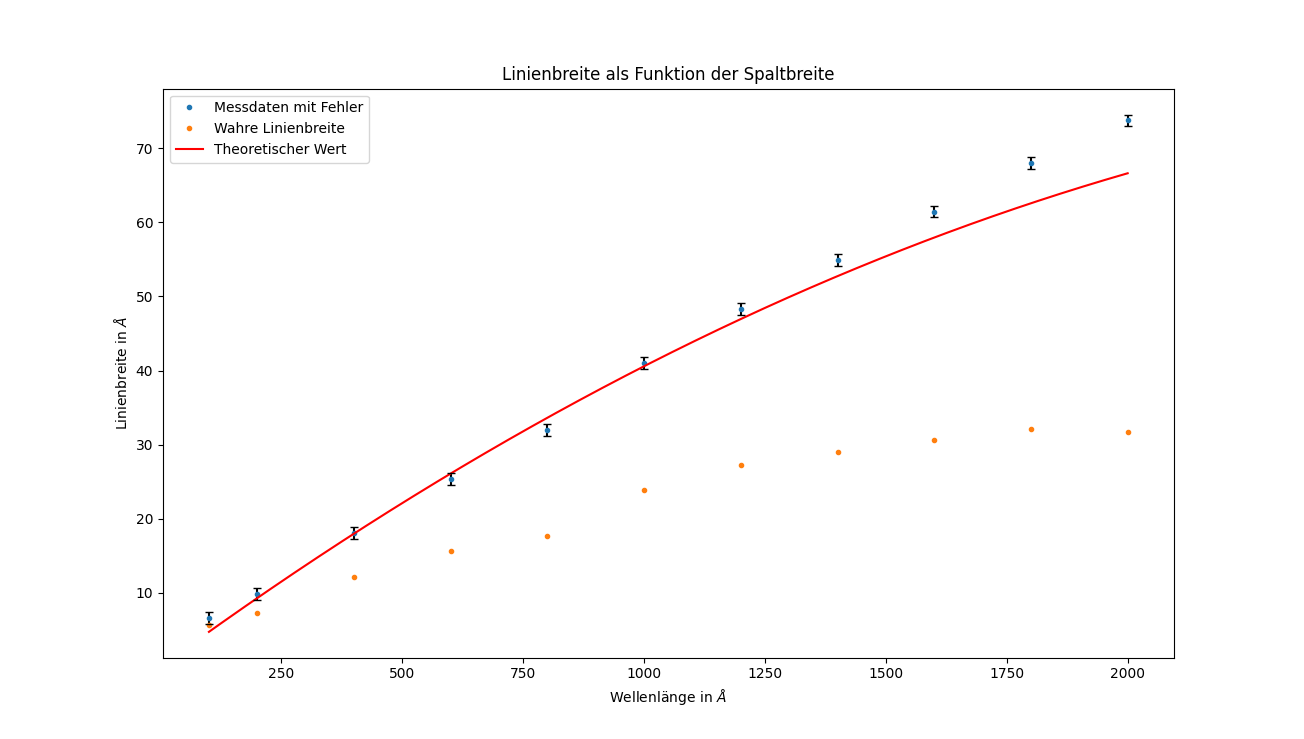
\includegraphics[width = \linewidth]{Bilder/Spaltbreite_Linie.png}
    \caption{Linienbreiten als Funktion der Spaltenbreite}
    \label{RealLin}
\end{figure}
Es fällt dabei auf, dass es einen massiven Unterschied zwischen "'Reale Linienbreite"`, theoretisch Berechneter und gemessener Linienbreite gibt. Die theoretische Liniennbreite wurde hier mit einem linearen 
Übergang zwischen der Annahme, dass es sich um ein Gauß-/Rechtechsintensitätsmuster handelt, erstellt. Am Anfang scheint diese Vorhersage sehr treffend zu sein. Gegen Ende hin weicht die Messung 
jedoch deutlich von dem theoretischen Wert ab. Das könnte unter anderem daran liegen, dass die Breite des Eingangsspaltes bei dieser Prognaose als vernachlässigbar klein angenommen wird. 
Dies trifft jedoch bei Spaltbreiten von fast 2mm nicht mehr zu. Der Unterschied zwischen "'Reale Linienbreite"` und Messwerten in dieser Größenordnung ist aus unserer Sicht schlichtweg nicht erklärbar.
Wahrscheinlich handelt es sich hier um einen Berechnungsfehler, genauer einen fehlenden Faktor zwei, der uns auch bei genaustem Hinschauen nicht aufgefallen ist. Multipliziert man den Realen Wert mit zwei 
erhält man nämlich Grafik \ref{Vergleich}.
\begin{figure}[h]
    \centering
    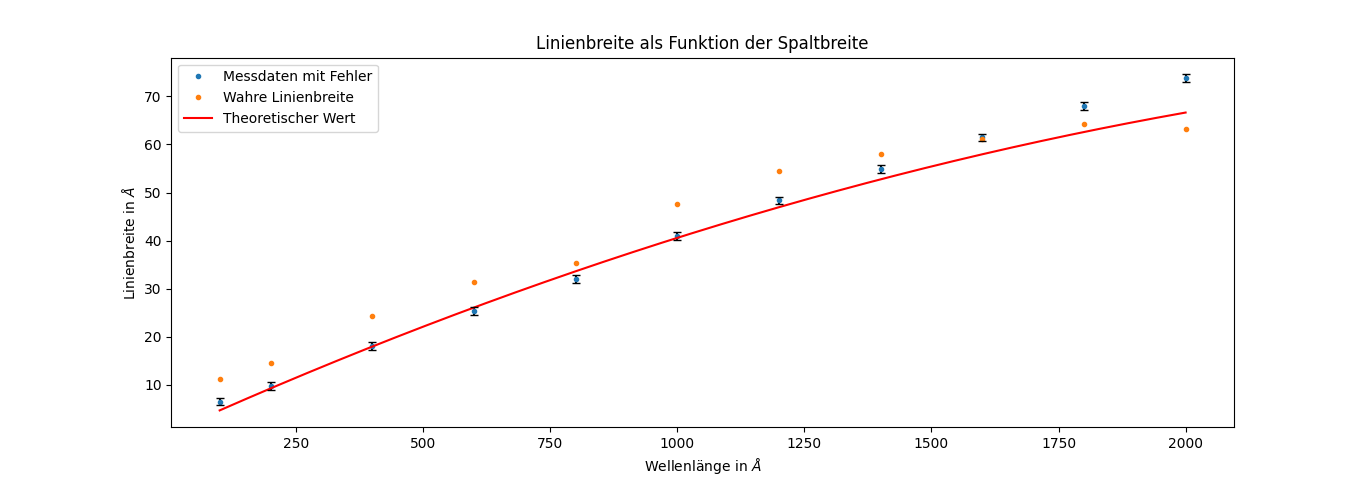
\includegraphics[width = \linewidth]{Bilder/Spaltbreite_Linie_vgl.png}
    \caption{Spekulation über einen Rechenfehler}
    \label{Vergleich}
\end{figure}

